\section{Configuration Spaces of Polygonal Chains}
\subsubsection{Configurations and Locked Configurations}
\subsection{Dissections}
\begin{prob}[Polygonal Dissection]\label{def:dissection}
Given two polygons of equal area, $P_1$ and $P_2$, partition $P_1$ into smaller
pieces,$\left\lbrace P_{1,i}\right\rbrace_{i=1}^n $, rearrange the pieces to
form $P_2$. \cite{frederickson1997dissections}
\end{prob}
\begin{figure}[h]
\begin{center}
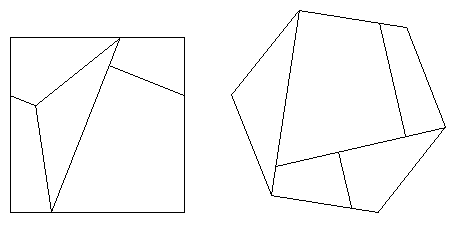
\includegraphics[scale=1]{graphics/polygonaldissection.png}
\caption{An axample of two polygons of equal area that can be rearranged into
the other by the given partition.\cite{davidEppstienJunkyard}}
\label{fig:polygonaldissection}
\end{center}
\end{figure}